\documentclass[11pt, a4paper, oneside]{article}

\usepackage{fontspec}
\setmainfont{Arial}
\usepackage[ngerman]{babel}
\usepackage{csquotes}
\usepackage{geometry}
\usepackage{setspace}
\usepackage{parskip}
\usepackage{titlesec}
\usepackage[hang, flushmargin]{footmisc}
\usepackage{fancyhdr}
\usepackage{xcolor}
\usepackage{graphicx}
\usepackage{pdfpages}
\usepackage[font=small, labelfont=bf, labelsep=colon]{caption}
\usepackage{subcaption}
\usepackage{booktabs}
\usepackage{tabularx}
\usepackage{longtable}
\usepackage{multirow}
\usepackage{tikz}
\usetikzlibrary{svg.path}
\usepackage{pgfplots}
\usepackage{siunitx}
\usepackage{listings}
\usepackage[printonlyused, withpage]{acronym}
\usepackage[backend=biber, style=apa, sorting=nyt, language=ngerman, apamaxprtauth=20]{biblatex}
\usepackage{hyperref}

\newcommand{\thesisType}{Bachelorarbeit}
\newcommand{\thesisInstitution}{IU University of Applied Sciences}
\newcommand{\thesisTitle}{Sandboxing MCP: Konzeption und Evaluation eines MCP Sandbox Layers zur Trust-Kalibrierung bei LLM-gestützten Änderungen in Low-Code-Plattformen}
\newcommand{\thesisAuthor}{Carl Ahrens}
\newcommand{\thesisMatrikel}{Matrikelnummer bis zur Abgabe zensiert}
\newcommand{\thesisAddressLineOne}{Straße Hausnummer bis zur Abgabe zensiert}
\newcommand{\thesisAddressLineTwo}{PLZ Ort bis zur Abgabe zensiert}
\newcommand{\thesisSupervisorOne}{Erstprüfer bis zur Abgabe zensiert}
\newcommand{\thesisSupervisorTwo}{Zweitprüfer bis zur Abgabe zensiert}
\newcommand{\thesisDate}{26.05.2026}
\newcommand{\thesisProgram}{Informatik (B.Sc.)}
\newcommand{\declarationFile}{figures/declaration-of-authenticity-signed.pdf}

\IfFileExists{config/layout-local.tex}{%
  \input{config/layout-local}
}{%
  \geometry{a4paper, top=2cm, bottom=2cm, left=2cm, right=2cm}
\onehalfspacing
\setlength{\parskip}{6pt}
\setlength{\parindent}{0pt}

\titleformat{\section}
{\normalfont\fontsize{12}{14.4}\bfseries\raggedright}
{\thesection}{1em}{}
\titleformat{\subsection}
{\normalfont\fontsize{12}{14.4}\bfseries\raggedright}
{\thesubsection}{1em}{}
\titleformat{\subsubsection}
{\normalfont\fontsize{12}{14.4}\bfseries\raggedright}
{\thesubsubsection}{1em}{}

\titlespacing*{\section}{0pt}{12pt}{12pt}
\titlespacing*{\subsection}{0pt}{12pt}{6pt}
\titlespacing*{\subsubsection}{0pt}{12pt}{6pt}

\setcounter{secnumdepth}{3}
\setcounter{tocdepth}{3}
\sloppy

\renewcommand{\footnotesize}{\fontsize{10}{12}\selectfont}

\pagestyle{fancy}
\fancyhf{}
\fancyfoot[C]{\thepage}
\renewcommand{\headrulewidth}{0pt}
\renewcommand{\footrulewidth}{0pt}
\fancypagestyle{plain}{%
  \fancyhf{}
  \fancyfoot[C]{\thepage}
  \renewcommand{\headrulewidth}{0pt}
}

}

% Code-Listings + eigene Commands
% Themes: Light (Default) und Dark - Umschalten via \codeDarkThemetrue
%
% Quellen für das Setup:
% - listings-Package: https://ctan.org/pkg/listings
% - VS Code Themes (Microsoft, MIT): github.com/microsoft/vscode/tree/main/extensions/theme-defaults/themes
% - TypeScript-Keywords aus der TS Language Spec

\definecolor{iuGreen}{RGB}{120, 190, 32}

% Theme-Toggle -> Default Light
\newif\ifcodeDarkTheme
\codeDarkThemefalse

% Light-Palette (VS Code Light+ leicht entsättigt für Print)
\definecolor{codeKeywordLight}{RGB}{0, 100, 170}
\definecolor{codeTypeLight}{RGB}{38, 127, 153}
\definecolor{codeStringLight}{RGB}{163, 21, 21}
\definecolor{codeCommentLight}{RGB}{100, 140, 80}
\definecolor{codeNumberLight}{RGB}{120, 120, 120}
\definecolor{codeFunctionLight}{RGB}{121, 94, 38}
\definecolor{codeIdentifierLight}{RGB}{0, 0, 0}
\definecolor{codeFrameLight}{RGB}{200, 200, 210}
\definecolor{codeBgTSLight}{RGB}{246, 248, 251}
\definecolor{codeBgJSLight}{RGB}{251, 250, 244}
\definecolor{codeBgJSONLight}{RGB}{248, 250, 246}
\definecolor{codeBgPyLight}{RGB}{247, 247, 250}
\definecolor{codeBgGenericLight}{RGB}{245, 245, 245}
\definecolor{codeHeaderBgLight}{RGB}{232, 236, 244}
\definecolor{codeHeaderTextLight}{RGB}{40, 60, 90}

% Dark-Palette (VS Code Dark+ dark_plus.json)
\definecolor{codeKeywordDark}{HTML}{569CD6}
\definecolor{codeTypeDark}{HTML}{4EC9B0}
\definecolor{codeStringDark}{HTML}{CE9178}
\definecolor{codeCommentDark}{HTML}{6A9955}
\definecolor{codeNumberDark}{HTML}{B5CEA8}
\definecolor{codeFunctionDark}{HTML}{DCDCAA}
\definecolor{codeIdentifierDark}{HTML}{D4D4D4}
\definecolor{codeFrameDark}{HTML}{3C3C3C}
\definecolor{codeBgTSDark}{HTML}{1E1E2E}
\definecolor{codeBgJSDark}{HTML}{1F1E1A}
\definecolor{codeBgJSONDark}{HTML}{1E1F1C}
\definecolor{codeBgPyDark}{HTML}{1F1F22}
\definecolor{codeBgGenericDark}{HTML}{1E1E1E}
\definecolor{codeHeaderBgDark}{HTML}{252526}
\definecolor{codeHeaderTextDark}{HTML}{9CDCFE}

% Aktive Theme-Farben
\ifcodeDarkTheme
  \colorlet{codeKeyword}{codeKeywordDark}
  \colorlet{codeType}{codeTypeDark}
  \colorlet{codeString}{codeStringDark}
  \colorlet{codeComment}{codeCommentDark}
  \colorlet{codeNumber}{codeNumberDark}
  \colorlet{codeFunction}{codeFunctionDark}
  \colorlet{codeIdentifier}{codeIdentifierDark}
  \colorlet{codeFrame}{codeFrameDark}
  \colorlet{codeBgTS}{codeBgTSDark}
  \colorlet{codeBgJS}{codeBgJSDark}
  \colorlet{codeBgJSON}{codeBgJSONDark}
  \colorlet{codeBgPy}{codeBgPyDark}
  \colorlet{codeBgGeneric}{codeBgGenericDark}
  \colorlet{codeHeaderBg}{codeHeaderBgDark}
  \colorlet{codeHeaderText}{codeHeaderTextDark}
\else
  \colorlet{codeKeyword}{codeKeywordLight}
  \colorlet{codeType}{codeTypeLight}
  \colorlet{codeString}{codeStringLight}
  \colorlet{codeComment}{codeCommentLight}
  \colorlet{codeNumber}{codeNumberLight}
  \colorlet{codeFunction}{codeFunctionLight}
  \colorlet{codeIdentifier}{codeIdentifierLight}
  \colorlet{codeFrame}{codeFrameLight}
  \colorlet{codeBgTS}{codeBgTSLight}
  \colorlet{codeBgJS}{codeBgJSLight}
  \colorlet{codeBgJSON}{codeBgJSONLight}
  \colorlet{codeBgPy}{codeBgPyLight}
  \colorlet{codeBgGeneric}{codeBgGenericLight}
  \colorlet{codeHeaderBg}{codeHeaderBgLight}
  \colorlet{codeHeaderText}{codeHeaderTextLight}
\fi

\graphicspath{{figures/}}
\pgfplotsset{compat=1.18}
\sisetup{locale=DE}
\renewcommand{\figurename}{Abb.}
\renewcommand{\tablename}{Tab.}

% TypeScript-Dialekt - listings kennt kein TS, Keywords aus der TS Language Spec
\lstdefinelanguage{TypeScript}{
  keywords={break, case, catch, class, const, continue, debugger, default, delete,
      do, else, enum, export, extends, false, finally, for, function, if,
      implements, import, in, instanceof, interface, let, new, null, package,
      private, protected, public, return, super, switch, this, throw, true,
      try, typeof, var, void, while, with, yield, async, await, from, as,
      readonly, abstract, namespace, type, satisfies, keyof, infer, declare, is},
  keywordstyle=\color{codeKeyword}\bfseries,
  ndkeywords={string, number, boolean, any, unknown, never, object, Promise, Array,
      Record, Partial, Pick, Omit, Map, Set, void, Buffer},
  ndkeywordstyle=\color{codeType}\bfseries,
  identifierstyle=\color{codeIdentifier},
  sensitive=true,
  comment=[l]{//},
  morecomment=[s]{/*}{*/},
  commentstyle=\color{codeComment}\itshape,
  stringstyle=\color{codeString},
  morestring=[b]',
  morestring=[b]",
  morestring=[b]`,
}

\lstdefinelanguage{JSONext}{
  keywords={true, false, null},
  keywordstyle=\color{codeKeyword}\bfseries,
  sensitive=true,
  string=[s]{"}{"},
  stringstyle=\color{codeString},
  comment=[l]{//},
  commentstyle=\color{codeComment}\itshape,
}

% Basis-Style für alle Code-Listings
\lstdefinestyle{codebase}{
basicstyle=\ttfamily\footnotesize\color{codeIdentifier},
backgroundcolor=\color{codeBgGeneric},
keywordstyle=\color{codeKeyword}\bfseries,
commentstyle=\color{codeComment}\itshape,
stringstyle=\color{codeString},
numberstyle=\tiny\color{codeNumber},
numbers=left,
numbersep=10pt,
breaklines=true,
breakatwhitespace=true,
columns=fullflexible,
keepspaces=true,
showstringspaces=false,
tabsize=2,
frame=single,
rulecolor=\color{codeFrame},
framerule=0.4pt,
framesep=4pt,
xleftmargin=14pt,
xrightmargin=4pt,
aboveskip=4pt,
belowskip=10pt,
captionpos=b,
upquote=true,
literate={ä}{{\"a}}1 {ö}{{\"o}}1 {ü}{{\"u}}1 {Ä}{{\"A}}1 {Ö}{{\"O}}1 {Ü}{{\"U}}1 {ß}{{\ss}}1 {…}{{...}}3
}

\lstdefinestyle{ts}{
  style=codebase,
  language=TypeScript,
  backgroundcolor=\color{codeBgTS},
}

\lstdefinestyle{js}{
  style=codebase,
  language=Java,
  backgroundcolor=\color{codeBgJS},
}

\lstdefinestyle{jsonext}{
  style=codebase,
  language=JSONext,
  backgroundcolor=\color{codeBgJSON},
}

\lstdefinestyle{pythonext}{
  style=codebase,
  language=Python,
  backgroundcolor=\color{codeBgPy},
}

\lstset{style=codebase}

% Pfad-Header über Code-Listing Nutzung zB: \codepath{backend/src/msl/core.ts}
\newcommand{\codepath}[1]{%
  \par\nopagebreak
  \noindent\colorbox{codeHeaderBg}{%
    \parbox{\dimexpr\linewidth-2\fboxsep\relax}{%
      \color{codeHeaderText}\ttfamily\footnotesize\strut #1\strut%
    }%
  }\par\nopagebreak\vspace{-2pt}%
}

\addbibresource{bibliography.bib}
\makeatletter
\renewcommand*{\apablx@ifrevnameappcomma}{\@secondoftwo}
\makeatother
\DefineBibliographyExtras{ngerman}{%
  \renewcommand*{\finalandcomma}{}%
}

\hypersetup{
  colorlinks=true,
  linkcolor=black,
  citecolor=black,
  urlcolor=codeKeyword,
  pdfauthor={\thesisAuthor},
  pdftitle={\thesisTitle},
  pdfsubject={Bachelorarbeit},
}

\newcommand{\todo}[1]{\textcolor{red}{\textbf{[TODO: #1]}}}
\newif\ifincludeListOfFigures
\includeListOfFiguresfalse
\newif\ifincludeListOfTables
\includeListOfTablesfalse


\begin{document}

\hypersetup{pageanchor=false}
\begin{titlepage}
    \thispagestyle{empty}

    \begin{center}

        \vspace*{0.5cm}
        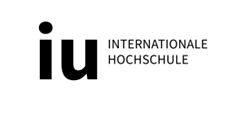
\includegraphics[width=6cm]{iu-logo}

        \vspace{2cm}

        {\fontsize{18}{21.6}\bfseries\selectfont \thesisType}

        \vspace{0.8cm}

        {\fontsize{11}{13.2}\selectfont
            \thesisInstitution\\[6pt]
            Studiengang: \thesisProgram}

        \vspace{2.5cm}

        {\fontsize{14}{18}\bfseries\selectfont
            \thesisTitle}

        \vspace{2.5cm}

        {\fontsize{11}{15}\selectfont
            \thesisAuthor\\[6pt]
            Matrikelnummer: \thesisMatrikel\\[6pt]
            \thesisAddressLineOne\\[6pt]
            \thesisAddressLineTwo}

    \end{center}

    \vfill

    {\fontsize{11}{15}\selectfont
        \noindent
        Betreuer: \thesisSupervisorOne\\[6pt]
        Zweitkorrekteur: \thesisSupervisorTwo\\[6pt]
        Abgabedatum: \thesisDate}

    \vspace{1cm}

\end{titlepage}

\clearpage
\hypersetup{pageanchor=true}

\pagenumbering{Roman}
\setcounter{page}{2}

\input{frontmatter/abstract}
\newpage

\tableofcontents
\newpage

\ifincludeListOfFigures
  \listoffigures
  \addcontentsline{toc}{section}{Abbildungsverzeichnis}
  \newpage
\fi

\ifincludeListOfTables
  \listoftables
  \addcontentsline{toc}{section}{Tabellenverzeichnis}
  \newpage
\fi

\section*{Abkürzungsverzeichnis}
\addcontentsline{toc}{section}{Abkürzungsverzeichnis}

\begin{acronym}[OWASP]
    \acro{MSL}{MCP Sandbox Layer}
    \acro{MCP}{Model Context Protocol}
    \acro{LLM}{Large Language Model}
    \acro{DSL}{Domain-Specific Language}
    \acro{API}{Application Programming Interface}
    \acro{SSE}{Server-Sent Events}
    \acro{SPA}{Single Page Application}
    \acro{BEM}{Block Element Modifier}
    \acro{OWASP}{Open Worldwide Application Security Project}
\end{acronym}

\newpage

\pagenumbering{arabic}
\setcounter{page}{1}

\input{chapters/01-einleitung}
\newpage
\input{chapters/02-grundlagen}
\newpage
\input{chapters/03-methodik}
\newpage
\input{chapters/04-konzeption}
\newpage
\input{chapters/05-evaluation}
\newpage
\input{chapters/06-diskussion}
\newpage
\input{chapters/07-fazit}

\newpage
\phantomsection
\printbibliography[heading=bibintoc, title={Literaturverzeichnis}]

\newpage
\appendix
\input{appendices/01-anhang}

\newpage
\section*{Disclaimer}
\addcontentsline{toc}{section}{Disclaimer}

\textbf{Erklärung zur Nutzung von KI-gestützten Werkzeugen}

Im Rahmen der Erstellung dieser Arbeit wurden KI-gestützte Werkzeuge unterstützend eingesetzt.
Hierbei wurden insbesondere ChatGPT (OpenAI, Modell GPT-5.3) sowie Claude (Anthropic, Modell Opus und Sonnet) verwendet.
Der Einsatz beschränkte sich auf folgende Bereiche:

\begin{itemize}
    \item \textbf{Softwareentwicklung:} KI-gestützte Code-Assistenz wurde unterstützend bei
          der Implementierung des Prototyps verwendet, insbesondere bei der Strukturierung
          von Code, der Erstellung von Boilerplate-Komponenten sowie bei der Fehlersuche.
          Sämtliche vorgeschlagenen oder erzeugten Codebestandteile wurden vom Autor geprüft,
          angepasst und inhaltlich verantwortet.

    \item \textbf{Textredaktion:} KI-Werkzeuge wurden punktuell zur sprachlichen Überarbeitung
          einzelner Passagen eingesetzt. Die fachliche Konzeption, inhaltliche Ausarbeitung,
          wissenschaftliche Argumentation und Analyse erfolgten eigenständig durch den Autor.
\end{itemize}

Die Verantwortung für den gesamten Inhalt dieser Arbeit - einschließlich aller fachlichen
Aussagen, der Methodik, der Ergebnisinterpretation sowie der Quellenarbeit - liegt
ausschließlich beim Autor.

\vspace{12pt}
\textbf{Hinweis zu fachlichen Vorüberlegungen und Praxisbezug}

Einzelne Architekturüberlegungen dieser Arbeit wurden durch allgemeine berufspraktische
Erfahrungen und eigene fachliche Vorüberlegungen des Autors mitinspiriert. Es wurden
jedoch keine nicht öffentlichen Unterlagen, Quellcodes, internen Dokumente oder
vertraulichen Informationen des Arbeitgebers in diese Arbeit übernommen.

\IfFileExists{\declarationFile}{%
    \includepdf[
        pages=-,
        pagecommand={\thispagestyle{plain}},
        addtotoc={1,section,1,Declaration of Authenticity,declaration}
    ]{\declarationFile}
}{%
    \section*{Declaration of Authenticity}
    \addcontentsline{toc}{section}{Declaration of Authenticity}

    I hereby declare that I have completed this Bachelors/ Master's thesis on my own and without
    any additional external assistance. I have made use of only those sources and aids specified and
    I have listed all the sources from which I have extracted text and content. This thesis or parts
    thereof have never been presented to another examination board. I agree to a plagiarism check
    of my thesis via a plagiarism detection service.

    \vspace{2cm}

    \begin{tabular}{p{6cm} p{6cm}}
        \rule{5cm}{0.4pt} & \rule{5cm}{0.4pt} \\
        Place, Date       & Student signature
    \end{tabular}
}


\end{document}
